\documentclass[9 pt]{beamer} %
\usetheme{Madrid}
\usepackage[latin1]{inputenc}
\usefonttheme{professionalfonts}
\usepackage{times}
\usepackage{tikz}
\usepackage{amsmath}
\usepackage{verbatim}
\usepackage{bbm}
 \usepackage{newlfont}
 \usepackage{nccmath}
\usepackage{scalerel}[2016-12-29]
\usepackage{appendixnumberbeamer} 
\usepackage{graphicx}
\def\stretchint#1{\vcenter{\hbox{\stretchto[440]{\displaystyle\int}{#1}}}}
\def\scaleint#1{\vcenter{\hbox{\scaleto[3ex]{\displaystyle\int}{#1}}}}
\usetikzlibrary{arrows,shapes}
 \def \r {{\rho}}
 \def \br {{\bar{\rho}}}
 \def \ber {{\bar{r}}}
  \def \tr {{\tilde{\rho}}}
\def \blue {\textcolor{blue}}
\def \red {\textcolor{red}}
\def \X {\mathcal{X}}
\def \F {\mathcal{F}}
\def \A {\mathcal{A}}
\def \bR {\mathbb{R}}
\def \bE {\mathbb{E}}
\def \bF {\mathbb{F}}

\def \bfR {\mathbf{R}}
\def \bfr {\mathbf{r}}
\def \bfx {\mathbf{x}}
\def \bfmu {\mathbf{\mu}}
\def \bfC {\mathbf{C}}
\def \bfe {\mathbf{e}}
\def \bfh {\mathbf{h}}


\def \O {\Omega}

\definecolor{MyDarkGreen}{rgb}{0.0,0.4,0.08}

%\del \bE {\mathbb{E}}

\author{Author}
\title{Presentation title}



\begin{document}

\title[Computational finance for option pricing]{Computational Finance and its implementation in Python with applications to option pricing }
\author{Andrea Mazzon}
%\date[\today]{ \today Z\"urich \\ \vspace{1cm} Joint work with F. Biagini and T. Meyer-Brandis}
\date{}
\institute[]{Ludwig Maximilians Universit\"at M\"unchen }


%%%%%%%%%%%%%%%%%%%%%%%%===Slide 0

\begin{frame}
\maketitle
\end{frame}



\begin{frame}{Main contents}
\tableofcontents
%\begin{itemize}
%\item Risk vs Uncertainty in the sense of Knight 
%\item Dispersion measures vs risk measures of downside risk
%\item Axiomatic theory of risk measures
%\item Computation of the required risk capital with risk measures
%\item Risk-adjusted performance measures
%\end{itemize}
\end{frame}

\section{Monte-Carlo method for option pricing and variance reduction techniques}
\frame{  \tableofcontents[
    sectionstyle=show/shaded,
    subsectionstyle=show/shaded/shaded,
    subsubsectionstyle=show/shaded/shaded/shaded
    ]}


\subsection{The Monte-Carlo method: motivation and a brief overview}
\frame{  \tableofcontents[
    sectionstyle=show/shaded,
    subsectionstyle=show/shaded/shaded,
    subsubsectionstyle=show/shaded/shaded/shaded
    ]}
    
 \begin{frame}{Motivation}
\begin{itemize}
\item A common problem we face in mathematical finance is the \blue{risk neutral valuation of a derivative}.
\item As you know, the \blue{price of a derivative} is expressed by the (possibly discounted) \blue{expectation of its payoff} at maturity, under a pricing measure (also called pricing, or martingale measure).
\item That is, \blue{we have to compute the expectation of a random variable}.
\item Problem: most often, there is \blue{no way to get an analytic formula} for the expectation of complex derivates, or even simpler derivatives written on underlying with non trivial dynamics. 
\item Broad idea: we can \blue{approximate the price by averaging} some possible, \blue{simulated realizations}  of the payoff.
\item The strong law of large numbers and some other convergence results may help us.
\end{itemize}
\end{frame}

    
 \begin{frame}{A bit more precisely..}
\begin{itemize}
\item Consider a random variable $X: \Omega \to \mathbb{R}^N$ defined on a probability space $(\Omega, \F, P)$. The probability measure $P$ may be viewed as a risk neutral measure.
\item Also consider a (payoff) function $f: \mathbb{R}^N \to \mathbb{R}$ such that $\text{Var}[f(X)] < \infty$. 
\item The aim is to compute the expectation
$$
\blue{\theta := \bE^P[f(X)] = \int_{\Omega}f(X)dP.}
$$
\item Suppose there is no analytic formula to derive $\theta$ above. We have to find an \red{approximation} $\hat \theta$.
\end{itemize}
\end{frame}  


 \begin{frame}{We can define independent drawings of $X$}
\begin{itemize}
\item Given $X: \Omega \to \mathbb{R}$ and $(\Omega, \F, P)$ as above, introduce:
\begin{align}
\tilde \Omega &:= \Omega \times \Omega \times \cdot \cdot  \times \Omega = \{ \tilde \omega= (\omega_1, \dots, \omega_n), \omega_i \in \Omega\},\notag \\
\tilde \F &:= \sigma( \F \times \F \times \cdot \cdot  \times \F),\notag \\
\tilde P\left(\prod_{i=1}^n A_i \right) &:= \prod_{i=1}^n P(A_i), \quad A_i \in \F.\notag
\end{align}
\item Also define the random variable $\tilde X = (\tilde X_1, \dots, \tilde X_n)$ by $\tilde X_i(\tilde \omega):= X(\omega_i)$. 
\item This is a way to see $\tilde  X(\tilde \omega)$ as \blue{$n$ different realizations $X(\omega_i)$}, $i=1,\dots,n$ of one random variable $X$, or as \red{one realization of $n$ i.i.d. random variables $\tilde X_i(\tilde \omega)$}, $i=1,\dots,n$.
\item This interpretation is at the base of the Monte-Carlo method, as it permits to  exploit the \red{Strong Law of Large Numbers}.
\item A similar construction and interpretation can be given for a $N$-dimensional random variable $X$.
\end{itemize}
\end{frame}    


\begin{frame}{Convergence results for sequences of i.i.d. random variables}
\begin{block}{Theorem: Strong Law of Large Numbers} 
\small{Let $(X_i)_{i \in \mathbb{N}}$ be i.i.d. integrable real valued random variables on  $(\Omega, \F, P)$, and set
$$
\mu := \bE^P[X_i], \quad i \in \mathbb{N}.
$$
Then 
$$
\lim_{n \to \infty} \frac{1}{n} \sum_{i=1}^n X_i = \mu \quad P-a.s.
$$}
\end{block}
\begin{block}{Theorem: Tschebyscheff Inequality} 
\small{Let $(X_i)_{i \in \mathbb{N}}$ be i.i.d. square integrable real valued random variables on  $(\Omega, \F, P)$, and set
$$
\mu := \bE^P[X_i], \quad \sigma^2:= \bE^P\left[(X_i-\mu)^2\right] ,\qquad i \in \mathbb{N}.
$$
Then for any $\epsilon, \delta >0$ we have
$$
P\left(\bigg | \frac{1}{n} \sum_{i=1}^n X_i - \mu \bigg | \ge \epsilon \right) \le  \frac{\sigma^2}{\epsilon^{2}n}.
$$
and
$$
P\left(\bigg | \frac{1}{n} \sum_{i=1}^n X_i - \mu \bigg | \ge  \frac{\sigma}{\delta^{1/2}n^{1/2}}\right) \le \delta.
$$}
\end{block}
\end{frame} 


\begin{frame}{Application to Monte-Carlo}
\begin{block}{Lemma} 
Let $(X_i)_{i \in \mathbb{N}}$ be a collection of i.i.d. integrable real valued random variables on  $(\Omega, \F, P)$, and let $f : \mathbb{R}^N \to \mathbb{R}$. Then the random variables $(f(X_i))_{i \in \mathbb{N}}$ are also i.i.d.
\end{block}
\begin{itemize}
\item The lemma above, together with the convergence results of the previous slide, allows us to approximate
 $$
\theta := \bE^P[f(X)] = \int_{\Omega}f(X)dP.
$$
by 
 $$
\hat \theta := \frac{1}{n} \sum_{i=1}^n f(X_i),
$$
where  $(X_i)_{i = 1, \dots, n}$ are independent realizations of $X$.
\item We can generate numerically $n$ realizations of a random variable $X$ with a given distribution $P^X$, starting from a sequence of (pseudo!) random numbers. 
\item One must give a \emph{seed}, i.e., a starting point for the pseudo-random numbers sequence.
\item The realizations will not be purely random, and not purely independent.
\end{itemize}
\end{frame} 

\begin{frame}{Pro and cons of Monte-Carlo}
\begin{itemize}
\item \blue{Pro:}
\begin{itemize}
\item It is very simple to understand and easy to implement.
\item The accuracy does not depend on the domain dimension (i.e., if we simulate $N$-dimensional  random variables the accuracy is the same).
\item The accuracy can be increased by just adding more valuations without loosing the previous estimates.
\item The function $f$ does not need to be continuous, but only square integrable.
\end{itemize}
\item \red{Cons:}
\begin{itemize}
\item Look at the Tschebyscheff Inequality: we only have a probabilistic bound. The worst case error is $\infty$.
\item The estimates depend on the generated random sequence. The sequence is not purely random. First, one has to find a good random number generator.
\end{itemize}
\item There are techniques that can be used to increase the accuracy. In the next slides we will see few of them.
\end{itemize}
\end{frame} 

\begin{frame}{Low-discrepancy sequences}
\small{
\begin{block}{Remark} 
 If $X$ has uniform distribution or has a cumulative distribution function $F$ which is easy to invert (in that case a realization $x_i$ can be generated as $x_i=F^{-1}(u_i)$, with $u_i$ realization of $U \sim U((0,1))$) then approximating $ \mathbb{E}[f(X)]$ reduces to approximate
 \begin{equation}\label{eq:integral}
\int_0^1 G(x)dx, 
 \end{equation} 
 for $G:[0,1] \to \mathbb{R}$.
 \end{block}
 \begin{block}{Theorem: Koksma-Hlawka inequality}
 If $G$ has bounded total variation on $(0,1)$, then for any points $x_1, \dots, x_n  \in (0,1)$ it holds
 $$
 \bigg| \frac{1}{n} \sum_{i=1}^n G(X_i) -  \int_0^1 G(x)dx \bigg| \le V(G)D^*(x_1, \dots, x_n),
 $$
 where 
 $$
 V(G)=\sup_S \sum_i|G(y_{i+1})-G(y_i)|
 $$
 over all partitions $S:= \{0=y_1<y_2<\dots<y_n=1\}$ and $D^*(x_1, \dots, x_n)$ is the star discrepancy
 $$
 D^*(x_1, \dots, x_n) = \sup_{b \in (0,1)} \Big| \frac{|\#\{x_i: 0 \le x_i \le b\}|}{n}  - b \Big|.
 $$
 \end{block}}
\end{frame} 

\begin{frame}{Low-discrepancy sequences}
\begin{itemize}
\item The result in the previous slide also holds for higher dimensions  (here we just wanted to simplify the notation).
\item It gives the motivation to look for low discrepancy sequences. 
\item Most well known low discrepancy sequences: Van der Corput, Halton, Sobol, Hammersley, Sobol, Niederreiter.
\item Here we don't focus on Low discrepancy sequences. A bit of references if you want to go deeper on this: 
\begin{itemize}
\item J. Dick and F. Pillichshammer, \emph{Digital Nets and Sequences. Discrepancy Theory and Quasi-Monte Carlo Integration}, Cambridge University Press, Cambridge, 2010
\item M. Drmota and R. F. Tichy, \emph{Sequences, discrepancies and applications}, Lecture Notes in Math., 1651, Springer, Berlin, 1997.
\item L. Kuipers,  H. Niederreiter, \emph{Uniform distribution of sequences}, Dover Publications, 2005.
\item \dots the course \emph{Numerical Methods for Financial Mathematics} at our master!
%\item Fries, Christian. \emph{Mathematical Finance: Theory, Modeling, Implementation}. John Wiley & Sons, 2007.
\end{itemize}
\item We focus instead on variance reduction techniques.
\end{itemize}
\end{frame} 


\subsection{Variance reduction techniques}
\frame{  \tableofcontents[
    sectionstyle=show/shaded,
    subsectionstyle=show/shaded/shaded,
    subsubsectionstyle=show/shaded/shaded/shaded
    ]}
    

\subsubsection{Introduction}
\frame{  \tableofcontents[
    sectionstyle=show/shaded,
    subsectionstyle=show/shaded/shaded,
    subsubsectionstyle=show/shaded/shaded/shaded
    ]}
    
\begin{frame}{Motivation - 1}
\begin{itemize}
 \item Consider a random variable $X: \Omega \to \mathbb{R}^N$ defined on a probability space $(\Omega, \F, P)$ and a (payoff) function $f: \mathbb{R}^N \to \mathbb{R}$ such that $\text{Var}[f(X)] < \infty$. 
 \item Monte-Carlo method: choosing $n \in \mathbb{N}$ large enough, we approximate
\blue{ $$
 \hat \mu := \frac{1}{n} \sum_{k=1}^n f(X_i) \approx \mu := \mathbb{E}^P[f(X)], 
 $$}
 where $(X_i)_{i = 1, \dots, n}$ are realizations of $X$, i.e., have same distribution as $X$.
 \item The estimator is of course \emph{unbiased}, i.e.,
\blue{$$
 \mathbb{E}^P\left[\hat \mu\right] = \mathbb{E}^P\left[\frac{1}{n} \sum_{k=1}^n f(X_i)\right] =\mathbb{E}^P\left[f(X)\right] =:\mu
 $$}
 \item We are \red{interested in} the variance of our estimator, i.e., in the quantity
 \red{$$
\text{Var}\left( \hat \mu\right)=\mathbb{E}^P\left[\left(\frac{1}{n} \sum_{k=1}^n f(X_i)- \mu\right)^2\right].
 $$}
 \end{itemize}
\end{frame}


\begin{frame}{Motivation - 2}
\begin{itemize}
\item We have seen that \blue{if $(X_i)_{i = 1, \dots, n}$ are independent}, we have convergence results for our estimator. Moreover, 
 \blue{$$
 \text{Var}\left( \hat \mu\right)= \mathbb{E}^P\left[\left(\frac{1}{n} \sum_{k=1}^n f(X_i)- \mu\right)^2\right] = \frac{1}{n}\text{Var}[f(X)].
 $$}
 \item It makes sense: the larger the number $n$ of simulated realizations of $X$, the smaller the variance of our estimator. 
 \item In particular, we have to increase the number of simulations by a factor of $C$ to reduce the standard deviation by a factor of $\sqrt{C}$.
 \item The question now is: can we do it better? 
 \item \red{Variance reduction techniques} aim to \red{reduce the variance of our estimator, without increasing the number of simulations.}
 \end{itemize}
\end{frame}

\begin{frame}{Some variance reduction techniques}
Three well known variance reduction techniques are:
\begin{itemize}
\item Antithetic variables
 \item Control variates
 \item Importance sampling
 \end{itemize}
 We will focus mostly on the first two techniques, together with applied examples. Here some references if you want to deepen Importance sampling:
 \begin{itemize}
\item A, Bouhari. \emph{Adaptative Monte Carlo Method, A Variance Reduction Technique}. Monte Carlo Methods and Their Applications. 10 (1): 1-24, 2004.
 \item P. J. Smith, M. Shafi, H. Gao. \emph{Quick simulation: A review of importance sampling techniques in communication systems}. IEEE Journal on Selected Areas in Communications. 15 (4): 597-613, 1997.
 \item Again, the course \emph{Numerical Methods for Financial Mathematics} at our master!
 \end{itemize}
\end{frame}


\subsubsection{Antithetic variables}
\frame{  \tableofcontents[
    sectionstyle=show/shaded,
    subsectionstyle=show/shaded/shaded,
    subsubsectionstyle=show/shaded/shaded/shaded
    ]}


\begin{frame}{Let's start from a simple result..}
\small{\begin{block}{Lemma}
Let $f, h: \mathbb{R} \to \mathbb{R}$ be two monotone functions, both increasing or both decraesing, and let $X: \Omega \to \mathbb{R}$ be a random variable defined on a probability space $(\Omega, \F, P)$.
Then
$$
\bE^P[f(X)h(X)] \ge \bE^P[f(X)]\bE^P[h(X)].
$$
\end{block}
\begin{block}{Proof}
The monotonicity assumption on $f$ and $h$ implies that for any $x,y \in \mathbb{R}$ we have
$$
\left(f(x)-f(y)\right)\left(h(x)-h(y)\right) \ge 0.
$$
Therefore, for any i.i.d. real valued random variables $X$ and $Y$ on $(\Omega, \F, P)$ it holds
$$
\left(f(X)-f(Y)\right)\left(h(X)-h(Y)\right)  \ge 0
$$
and then
$$
\bE \left[\left(f(X)-f(Y)\right)\left(h(X)-h(Y)\right)\right]  \ge 0,
$$
so that
$$
\bE \left[f(X)h(X)\right]+\bE \left[f(Y)h(Y)\right] \ge \bE \left[f(Y)h(X)\right]+\bE \left[f(X)h(Y)\right].
$$
Since $X$ and $Y$ are identically distributed, it follows that
$$
2\bE \left[f(X)h(X)\right]\ge 2 \bE \left[f(Y)h(X)\right],
$$
and since they are also independent, this implies that
$$
\bE^P[f(X)h(X)] \ge \bE^P[f(X)]\bE^P[h(X)].
$$
\end{block}}
\end{frame}

\begin{frame}{An interesting consequence}
\begin{block}{Proposition}
Let $f: \mathbb{R} \to \mathbb{R}$ be a monotone function, and $X: \Omega \to \mathbb{R}$ a random variable defined on a probability space $(\Omega, \F, P)$.
Then
$$
\text{Cov}[f(X),f(-X)] \le 0.
$$
\end{block}
\begin{block}{Proof}
We have that 
$$
\text{Cov}[f(X),f(-X)] = \bE^P[f(X)f(-X)]-\bE^P[f(X)]\bE^P[f(-X)].
$$
The result then follows since a direct application of the Lemma of the previous slide with $h(x):=-f(-x)$ implies that
$$
\bE^P[f(X)]\bE^P[f(-X)] \ge \bE^P[f(X)f(-X)]
$$ 
\end{block}
\end{frame}


\begin{frame}{Application to Monte-Carlo}
\small{
\begin{itemize}
\item Let $f: \mathbb{R} \to \mathbb{R}$ be a monotone function, and let $X: \Omega \to \mathbb{R}$ be a \red{symmetric} random variable defined on a probability space $(\Omega, \F, P)$.
\item From the last proposition we know that
$$
\text{Cov}[f(X),f(-X)] \le 0.
$$
\item Idea: choose $n$ even and generate $n/2$ realizations of $X$, call them $(X_i)_{i=1,\dots,n/2}$. Then define $X_{n/2+i}:=-X_i$,  $i=1,\dots,n/2$.
\item Since $X$ is symmetric, the estimator is unbiased:
$$
\blue{\bE[\hat \mu] }=  \frac{1}{n}  \bE\left[\sum_{k=1}^{n/2} f(X_i) + \sum_{k=1}^{n/2} f(-X_i)\right] = \frac{1}{n}\left( \sum_{k=1}^{n/2} \bE[f(X_i)] +\sum_{k=1}^{n/2} \bE[f(-X_i)] \right) \blue{= \mu}.
$$
\item What about the variance?
\begin{align}
\blue{\text{Var}[\hat \mu]} &= \frac{1}{n^2}\text{Var}\left[\sum_{k=1}^{n/2} f(X_i) + \sum_{k=1}^{n/2} f(-X_i)\right] \notag \\ &=  \frac{1}{n^2}\left(n \text{Var} [f(X)] + \text{Cov}\left(\sum_{k=1}^{n/2} f(X_i),\sum_{k=1}^{n/2} f(X_i)\right) \right) \notag \\
&=\frac{1}{n}\text{Var} [f(X)] +  \frac{1}{n}\text{Cov} [f(X),f(-X)] \blue{\le \frac{1}{n}\text{Var} [f(X)]}.  \notag 
\end{align}
\end{itemize}}
\end{frame}


\begin{frame}{Application to Monte-Carlo}
\begin{itemize}
\item To recap: if $X$ is symmetric, then setting $X_{n/2+i}:=-X_i$ for  $i=1,\dots,n/2$ gives us an unbiased estimator $\hat \mu$ such that
$$
\text{Var}[\hat \mu] \le \frac{1}{n}\text{Var} [f(X)].
$$
\item But $ \frac{1}{n}\text{Var} [f(X)]$ is the variance of the classical estimator, when we generate $n$ i.i.d. realizations of $X$! 
\item In this way, we reduce the variance of the estimator.
\item This approach is known as Antithetic variables.
\end{itemize}
\end{frame}


\begin{frame}{Antithetic variables for not symmetric $X$}
\begin{itemize}
\item Let $f: \mathbb{R} \to \mathbb{R}$ be a monotone function, and let $X: \Omega \to \mathbb{R}$ be a random variable defined on a probability space $(\Omega, \F, P)$. 
\item Suppose $X$ to be not symmetric. How can we apply Antithetic variables to reduce the variance of our estimator?
\item Call $F$ the cumulative distribution function of $X$. Suppose that we know (at least a good approximation of) $F^{-1}$.
\item Well known result: let $U \sim \text{Unif}(0,1)$ and define $Y:=F^{-1}(X)$. Then $X$ and $Y$ have same distribution.  
\item Let $U \sim \text{Unif}(0,1)$. Because of the result above, we have
$$
\bE^P[f(X)]=\bE^P[h(U)]
$$
with $h(x)=f \circ F^{-1}$.
\item Since $U$ is symmetric, we can approximate $\bE^P[h(U)]$ by Antithetic variables.
\end{itemize}
\end{frame}


\begin{frame}{Example: valuation of a call option  under Black-Scholes}
\begin{itemize}
\item We want to test the benefits of using Antithetic variables in the valuation of a call option under the Black-Scholes model.
\item This is indeed a case when we have of course the benchmark of the analytic formula for a call option.
\item In particular, we want to approximate the expectation $\bE^P[f(X_T)]$ for $T>0$, in the case when
$$
g(x)=(x-K)^+
$$
with $K>0$ and $X=(X_t)_{0 \le t \le T}$ is a stochastic process with initial value $X_0=x_0$ and dynamics
$$
dX_t = r X_t dt + \sigma X_t dW_t, \quad 0 \le t \le T,
$$
where $W=(W_t)_{0 \le t \le T}$ is $P$-Brownian motion.
\item Interpretation: $r$ is the risk free rate and $P$ is the martingale measure, i.e., the probability measure under which the discounted process $(e^{-r t}X_t)_{0 \le t \le T}$ is a martingale.
\end{itemize}
\end{frame}


\begin{frame}{Valuation with Antithetic variables}
\begin{itemize}
\item The problem reduces to the valuation of the expectation
$$
\bE^P[g(X-K)^+]
$$
where $X$ is the random variable
$$
X = X_0 e^{(r-\sigma^2)T + \sigma \sqrt{T} Z},
$$
with $ Z \sim \mathcal{N}(0,1)$.
\item That is, we have to valuate 
$$
\bE^P\left[f(Z)\right]
$$
where
$$
f(z)=\left(X_0 e^{(r-\sigma^2)T + \sigma \sqrt{T} z} - K \right)^+.
$$
\item So, we have a function of a symmetric random variable! We can directly use Antithetic variables.
\item We simulate $n/2$ realizations $(z_i)_{i=1,\dots,n/2}$ of a standard normal random variable and then define $z_{i+n/2}=-z_i$, $i=1,\dots,n/2$.
\end{itemize}
\end{frame}


\begin{frame}{Implementation with Python}
\begin{itemize}
\item In the Python package 
\begin{center}
\texttt{montecarlovariancereduction.antitheticvariables}
\end{center}
you can find the code relative to the comparison of Antithetic variables against the standard Monte-Carlo method.
\item In particular, in the class \texttt{GenerateBlackScholes} we generate the values of 
$$
X = X_0 e^{(r-\sigma^2)T + \sigma \sqrt{T} Z},
$$
starting from the ones of $Z$. We do this using both the standard Monte-Carlo approach and the Antithetic variables approach illustrated in the previous slide.
\item  Note that the method
\begin{center}
\texttt{numpy.random.standard\_normal(n)}
\end{center}
generates $n$ returns of a standard normal random variable. In this case, we give no seed: it will be different every time this method is called.
\end{itemize}
\end{frame}
 
 
 \begin{frame}{Experiment and results}
  In  
  \begin{center}
\texttt{antitheticVariablesTest}
\end{center}
and
\begin{center}
\texttt{compareStandardMCWithAV}
\end{center}
we do the following experiment:
\begin{itemize}
\item We fix the parameters $X_0=K=100$, $T=3$, $r=0.05$, $\sigma=0.5$.
\item For any number of simulations $n=10^3$, $10^4$, $10^5$ and $10^6$, we perform $100$ different valuations of the price of the call option, both with the standard and the Antithetic variables Monte-Carlo method. 
\item We then compute the average percentage error for both the methods.
\end{itemize}
The following table illustrates the results
\begin{table}[H]
 \begin{tabular}{|c|c|c|c|c|c|}
 \hline
& $n=10^3$ & $n=10^4$ & $n=10^5$ &  $n=10^6$\\
  \hline
  av. $\%$ error standard MC  & $6.25$ & $2.07$ & $0.59$ &  $0.20$    \\
 \hline
   av. $\%$ error AV & $5.51$ & $1.77$ & $0.53$ &  $0.17$   \\
\hline
\end{tabular}
\end{table}
\end{frame}

\subsubsection{Control variates}
\frame{  \tableofcontents[
    sectionstyle=show/shaded,
    subsectionstyle=show/shaded/shaded,
    subsubsectionstyle=show/shaded/shaded/shaded
    ]}


\begin{frame}{Setting and motivation}
\begin{itemize}
\item Let $X, Y: \Omega \to \mathbb{R}$ be two random variables defined on a probability space $(\Omega, \F, P)$.
\item Suppose you know the analytic value of 
$$
a:= \bE^P[X], \qquad \sigma_{X}^2 := \text{Var}[X], \qquad \sigma_{XY}:=\text{Cov}[X, Y],
$$
and also suppose $\sigma_{XY}>0$. 
\item Assume you want to approximate 
$$
b:=\bE^P[Y]
$$
\item The goal is to find an unbiased estimator of $b$ which has low variance.
\end{itemize}
\end{frame}


\begin{frame}{Control variates}
\begin{itemize}
\item Idea: simulate $n$ realizations $(x_i, y_i)$, $i=1,\dots,n$, of $(X,Y)$. Compute then
$$
\hat a := \frac{1}{n}\sum_{i=1}^n x_i, \qquad \hat b := \frac{1}{n}\sum_{i=1}^n y_i.
$$ 
\item Note that 
$$
\text{Cov}[\hat a, \hat b]=\frac{1}{n} \sigma_{XY}.
$$
\item What about an estimator 
\blue{$$
\hat b_{CV}:= \hat b - \beta(\hat a - a)
$$}
for a given $\beta>0$?
\item It is unbiased:
$$
\bE^P[\hat b_{CV}] = \bE^P[\hat b] + \beta \bE^P[\hat a - a] = b.  
$$
\item What about the variance? 
$$
\text{Var}[\hat b_{CV}] = \frac{1}{n} \sigma_{Y}^2 + \beta^2  \frac{1}{n} \sigma_{X}^2 -2\beta \frac{1}{n} \sigma_{XY}.
$$
\item It is minimized by \blue{$\beta=\frac{\sigma_{XY}}{\sigma_X^2}$}. For such a value of $\beta$, we find
\blue{$$
\text{Var}[\hat b_{CV}] = \text{Var}[\hat b] -  \frac{1}{m}\frac{\sigma_{XY}^2}{\sigma_X^2}.
$$}
\end{itemize}
\end{frame}

\section{Option pricing under the Binomial model}
\frame{  \tableofcontents[
    sectionstyle=show/shaded,
    subsectionstyle=show/shaded/shaded,
    subsubsectionstyle=show/shaded/shaded/shaded
    ]}

\subsection{Motivation and setting}
\frame{  \tableofcontents[
    sectionstyle=show/shaded,
    subsectionstyle=show/shaded/shaded,
    subsubsectionstyle=show/shaded/shaded/shaded
    ]}
    
\begin{frame}{Motivation}
The multi-period Binomial model for option pricing is widely used by practitioners in financial applications mainly because:
\begin{itemize}
\item It is very easy to understand and simulate.
\item It is particularly convenient to price options involving a choice of the holder, like American and Bermudan options.
\item It approximates the Black-Scholes model when the length of the periods tends to zero.
\item Option pricing is not based on pure Monte-Carlo techniques but relies on weighting the payoff relative to any scenario by the (analytic!) probability of the scenario.
\end{itemize}
\end{frame}

\begin{frame}{The setting}
\begin{itemize}
 \item Consider a multi-period model with times \red{$t=0,1,\dots,T$}, and consider a \red{probability space $(\O,\F,\bF,P)$}, where $\bF=(\F_t)_{t=0,\dots,T}$ is a filtration representing information.
 \item Suppose there exist:
\begin{itemize}
\item A \red{risk free asset} defined by \blue{$S_t^0 = (1+\rho)^t$}, $t=0,\dots,T$, with a deterministic interest rate $\rho>0$.
\item A \red{risky asset} adapted to $\bF$ defined by 
$$
\blue{S_t=S_0\cdot Y_1 \cdot \dots \cdot Y_t, \quad t=1,\dots,T,}
$$
where \blue{$Y_t$ can take the two values $d$, $u$ with $0<d<1+\rho<u$}, for any $t=1,\dots,T$, and \blue{$(Y_t)_{t=1,\dots,T}$ are i.i.d. and such that $Y_{t+1}$ is independent of $\F_t$}.
\end{itemize}
\item It then holds
\begin{align}
&\blue{S_t^0=S^0_{t-1}(1+\rho)}, \quad t=1,\dots,T\notag \\
\intertext{and}
&\blue{S_t=S_{t-1}Y_t}, \quad t=1,\dots,T.\notag
\end{align}
\end{itemize}
\end{frame}

\begin{frame}{Admissible strategies}
At every time $t=0,\dots,T-1$, an investor can construct a \red{portfolio of value $V_t$}, trading on the risk-free asset $S^0$ and on the risky asset $S$.
\begin{itemize}
\item The value of the portfolio is given by
$$
\blue{V_t = \alpha_t S_t + \beta_t S_t^0}, \quad t=1,\dots, T,
$$
where $(\alpha_t)_{t=1,\dots,T}$ and $(\beta_t)_{t=1,\dots,T}$ are $\bF$-predictable, discrete process.

\item The strategy $(\alpha, \beta)$ must be \red{self-financing}: it must hold
$$
\blue{V_t =   \alpha_{t} S_t + \beta_{t} S_t^0 =  \alpha_{t-1} S_t + \beta_{t-1} S_t^0}, \quad t=1,\dots,\quad T.
$$
\end{itemize}
\end{frame}

\begin{frame}{Arbitrage theory}
\begin{block}{Definition}A portfolio $V$ is an \red{arbitrage} if:
\begin{itemize}
\item $V$ is obtained by a self-financing and predictable strategy;
\item $P(V_0=0)=1$;
\item $P(V_t \ge 0)=1$ and  $P(V_t > 0)>0$ for some $t$.
\end{itemize}
\end{block}

\begin{block}{Proposition}
The market is \red{arbitrage free} \blue{only if}  \red{$d < 1 + \rho <u$}.
\end{block}
\begin{itemize}
\item Suppose \blue{$1 + \rho \le d < u$}, and consider the self-financing portfolio defined by
$$
V_t = S_t - \frac{S_0}{S_0^0} S^0_t,  \quad t=0,1,\dots, T.
$$ 
Then we have $V_0=0$ and 
$$
V_1=S_1- \frac{S_0}{S_0^0}S_1^0\ge S_0d-S_0(1+\rho) \ge 0.
$$
\item If \blue{$d<u\le 1+\rho$}, changing the signs to the strategy above leads to an arbitrage
\end{itemize}
\end{frame}

\begin{frame}{Equivalent martingale measure}
In order for the market to be arbitrage-free and complete, \red{there must exist a unique measure $Q \sim P$ such that $\frac{S}{S^0}$ is a martingale}, i.e., such that
\begin{equation}\label{eq:martingale}
\bE^Q\left[\frac{S_{t+1}}{S^0_{t+1}}\big|\F_t\right]=\frac{S_{t}}{S^0_{t}}, \quad t=0,\dots,T-1.
\end{equation}
Note that the measure $Q$ is identified by the probability $q:=P(Y_t=u)$.

Since
$$
\bE^Q\left[\frac{S_{t+1}}{S^0_{t+1}}\big|\F_t\right] =\frac{(qu+(1-q)d)S_t}{S_t^0(1+\rho)}, \quad t=0,\dots,T-1,
$$
equation \eqref{eq:martingale} holds if and only if $qu+(1-q)d=1+\rho$, that is,
$$
\red{q=\frac{1+\rho-d}{u-d}.}
$$
Such $Q$ exists and is unique as we have supposed $0<d<1+\rho<u$, and 
$$
\blue{\frac{dQ}{dP}(\omega)=\left(\frac{q}{p}\right)^{n(\omega)}\left(\frac{1-q}{1-p}\right)^{T-n(\omega)},}
$$
where \blue{$p:=P(Y_t=u)$} and \blue{$n(\omega)$ is the number of times} $t=1,\dots,T$ when \blue{$Y_t(\omega)=u$}.
\end{frame}


\begin{frame}{Replicating strategy}
\begin{itemize}
\item Assume we want to \red{find an admissible strategy $(\alpha_t,\beta_t)$, $t=0, \dots, T$, such that the value of the portfolio
$$
\alpha_t S_t + \beta_t(1+\rho)^t
$$
equals the value $V_t$  of an option} at every time  $t = 0, \dots, T$.
\item From now on, fix $t=1,\dots,T$, and suppose we know $S_{t-1}$.
\item Call $V_t^u$ the value of the option at time $t$ when $Y_t=u$ and $V_t^d$ the value of the option at time $t$ when $Y_t=d$. 
\item It must hold
$$
\begin{cases}
\alpha_t u S_{t-1} + \beta_t (1+\rho)^t = V_t^u,\\
\alpha_t d S_{t-1} + \beta_t (1+\rho)^t = V_t^d.
\end{cases}
$$
\item The solution to the system above is
\blue{\begin{align}
\alpha_t &= \frac{V_t^u-V_t^d}{S_{t-1}(u-d)},\notag \\
\beta_t &= \frac{uV_t^d-dV_t^u}{(1+\rho)^t(u-d)}.\notag
\end{align}}
and gives the right replicating strategy.
\end{itemize}
\end{frame}


\begin{frame}{Option pricing from admissibility}
\begin{itemize}
\item Remember that our strategy $(\alpha_t,\beta_t)$, $t=0, \dots, T$, has to be admissible!
\item This means that we must have that
\begin{align}
\blue{V_{t-1}}&=\alpha_{t-1} S_{t-1} + \beta_{t-1}(1+\rho)^{t-1}\notag \\
&=\alpha_{t} S_{t-1} + \beta_{t}(1+\rho)^{t-1}\notag \\
&=\frac{V_t^u-V_t^d}{u-d}+ \frac{uV_t^d-dV_t^u}{(1+\rho)(u-d)}\notag \\
&=\frac{(1+\rho)(V_t^u-V_t^d)+uV_t^d-dV_t^u}{(1+\rho)(u-d)}\notag \\
&=\frac{(1+\rho-d)V_t^u+(u-1-\rho)V_t^d}{(1+\rho)(u-d)}\notag \\
&=\frac{qV_t^u+(1-q)V_t^d}{1+\rho}\notag \\
&\blue{=\frac{1}{1+\rho}\bE^Q[V_t|\F_{t-1}]}\notag.
\end{align}
\item Then we have that \red{the value $(V_t)_{t=0,\dots,T}$ of the option is a martingale under $Q$}.
\item This gives us a pricing theorem.
\end{itemize}
\end{frame}


\begin{frame}{Option pricing}
\begin{block}{Theorem}
The value $V_0$  of a contingent claim with maturity $T$ and payoff $V_T$ depending on the realizations of $S$ until time $T$, is given by
$$
V_0=\frac{1}{(1+\rho)^T}\bE^Q[V_T].
$$
\end{block}

\begin{block}{Remark}
Because of the theorem above, we always simulate our Binomial model under the risk neutral measure $Q$.
\end{block}
\end{frame}

\subsection{Simulation of the Binomial model}
\frame{  \tableofcontents[
    sectionstyle=show/shaded,
    subsectionstyle=show/shaded/shaded,
    subsubsectionstyle=show/shaded/shaded/shaded
    ]}
    
\begin{frame}{Motivation}
\begin{itemize}
\item Our main goal here is to get the price of European and (most importantly) American options written on an underlying Binomial model. 
\item This valuation will approximate the price of the options written on an underlying log-normal model.
\item We then simulate the realizations of the underlying model in Python, and get the payoff on the realizations, along with its expectation.
\item Remember we have to price under the risk neutral measure $Q$: then we simulate the realizations of the process under $Q$.
\item The most naive way we can imagine to do this is a brute force Monte-Carlo approximation..
\end{itemize}
\end{frame}


\begin{frame}{Monte-Carlo method}
\begin{itemize}
\item Imagine we want to valuate the discounted price of an European option with a given payoff function $f:\mathbb{R} \to \mathbb{R}$, written on the process $S$, with maturity $T$.
\item Suppose  we don't know any analytic formula in order to derive the price as  $$V_0=\frac{1}{(1+\rho)^T}\bE^Q[f(S_T)].$$
\item We consider \red{$N$ \emph{states of the world} $\omega_1, \omega_2, \dots, \omega_N \in \Omega$}.
\item To any $\omega_1, \omega_2, \dots, \omega_N$, we associate a given trajectory of the process $(S_t)_{t = 0, \dots,T}$, with dynamics given under the measure $Q$. 
\item In particular, we suppose that the trajectories
$(\red{S_t(\omega_k)})_{t = 0, \dots,T},$ $k=1,2,\dots,N$ are \red{independent} of each other.
\item Strong law of large numbers:
$$
 \frac{1}{n}\sum_{k=1}^n f(S_T(\omega_k)) \to \bE^Q[f(S_T)] \quad \text {a.s., when $n \to \infty$}.
$$
\item The idea is to simulate such trajectories and approximate
\blue{$$
\bE^Q[f(S_T)] \approx \frac{1}{N}\sum_{k=1}^N f(S_T(\omega_k)).
$$}
\end{itemize}
\end{frame}


\begin{frame}{Monte-Carlo method for the Binomial model}
\begin{itemize}
\item Our first goal is then to generate a sequence of random numbers in order to simulate $N$ independent trajectories $(S_t(\omega_k))_{t = 0, \dots,T},$ $k=1,2,\dots,N$ of $S$ under the risk neutral measure $Q$, and store them in a $(T+1) \times N$ matrix.
\item First (not that) bad news: it is not possible to generate a sequence of perfectly random numbers, the best we can get is a sequence of \emph{pseudo}-random numbers.
\item Idea: \red{generate} (with the help of Python in our case) a sequence of $T \cdot N$ \red{uniformly distributed, pseudo-random numbers $0 < x_{i,j} < 1$}, $i=1,\dots,T$, $j=1,\dots,N$. 
\item Fix $\rho>0$, $u>1+\rho$, $d<1$, $q=\frac{1+\rho-d}{u-d}.$ 
\item For every $i=1,\dots,T$, $j=1,\dots,N$, define 
\blue{$$
Y_{i}(\omega_j)=
\begin{cases}
u \quad \text{if $x_{i,j} <q$}\\
d \quad \text{if $x_{i,j} \ge q$}
\end{cases}
$$}
and
\blue{$$
S_{i+1}(\omega_j)=Y_{i}(\omega_j)S_{i}(\omega_j).
$$}
\end{itemize}
\end{frame}

\begin{frame}{Implementation in Python}
\begin{itemize}
\item You can find the code relative to the simulation of the Binomial model with the pure Monte-Carlo approach described above in
\begin{center}
\texttt{binomialmodel.creationandcalibration.binomialModelMonteCarlo}
\end{center}
\item Note that the class you find there extends the one in
\begin{center}
\texttt{binomialmodel.creationandcalibration.binomialModel}.
\end{center}
\item This is done in order to implement in the parent class some methods that do not strictly depend on the way in which we simulate the process.
\item In this way, we don't have to copy and paste these methods in every class where we simulate the model in some way: object oriented programming feature.
\end{itemize}
\end{frame}


\begin{frame}{Some paths}
\begin{itemize}
\item We plot below some paths of the Binomial model.
\item In the figure at the left we take $S_0=3$, $u=1.1$, $d=0.9$, $r=0.05$, $T=150$, having then $q=\frac{1+\rho-d}{u-d}=0.75$. 
\item On the right, $S_0=3$, $u=2$, $d=0.5$, $r=0.1$, $T=150$, $q=\frac{1+\rho-d}{u-d}=0.4$.
\end{itemize}
 \begin{figure}
\centering
\begin{minipage}[b]{.5\textwidth}
  \centering
 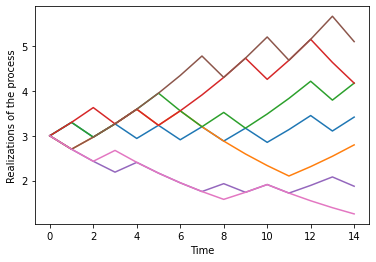
\includegraphics[scale=0.4]{pathsu11.png}
\end{minipage}%
\begin{minipage}[b]{.5\textwidth}
  \centering
 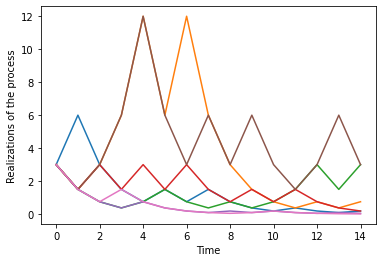
\includegraphics[scale=0.4]{pathsu2.png}
\end{minipage}
\end{figure}
\end{frame}

\begin{frame}{A first test}
We show here the evolution of the discounted average of the process and of the probability $Q(S_{t_j}>(1+\rho)^{t_j}S_0)$, computed by using the Monte-Carlo method with $10^5$ simulations, for $S_0=3$, $u=1.1$, $d=0.9$, $r=0.05$, $T=150$. In this case, we have $q=\frac{1+\rho-d}{u-d}=0.75$.
 \begin{figure}
\centering
\begin{minipage}[b]{.5\textwidth}
  \centering
 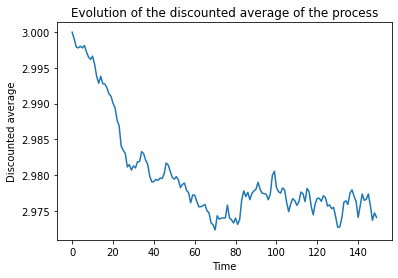
\includegraphics[scale=0.4]{Averaged09u11r005.png}
\end{minipage}%
\begin{minipage}[b]{.5\textwidth}
  \centering
 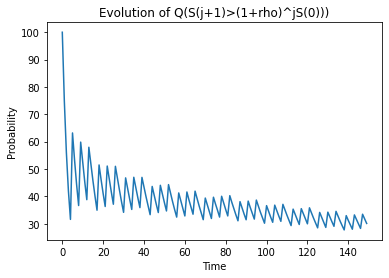
\includegraphics[scale=0.4]{Probabilityu11d09.png}
\end{minipage}
\end{figure}
\end{frame}


\begin{frame}{But something can go wrong..}
Look at the evolution of the same quantities, again computed by using the Monte-Carlo method, choosing now $S_0=3$, $u=2$, $d=0.5$, $r=0.1$, $T=150$, $q=\frac{1+\rho-d}{u-d}=0.4$.
 \begin{figure}
\centering
\begin{minipage}[b]{.5\textwidth}
  \centering
 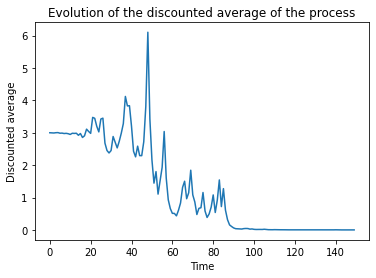
\includegraphics[scale=0.4]{Averaged05u2r01.png}
\end{minipage}%
\begin{minipage}[b]{.5\textwidth}
  \centering
 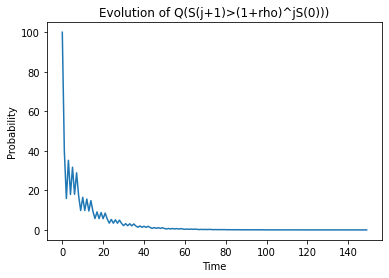
\includegraphics[scale=0.4]{Probabilityu2d05.png}
\end{minipage}
\end{figure}
\end{frame}


\begin{frame}{Why is the estimate of the average that inaccurate?}
\begin{itemize}
\item The anaytic average of the discounted process is equal to $S_0$, due to many realizations such that $S_{t_j}<(1+\rho)^{t_j}S_0$ and few, extremely high realizations. 
\item If you buy $S$ at time $t=0$, and you hold it for $150$ time steps, you make a positive gain with a very low probability, but the gain can be extremely high.
\item  \red{Problem:} The approximated average is strongly impacted by whether or not those paths leading to high gains are simulated or not.
\end{itemize}
\end{frame}

\begin{frame}{Let's choose two different seeds, for the same parameters}
 \begin{figure}
\centering
\begin{minipage}[b]{.5\textwidth}
  \centering
 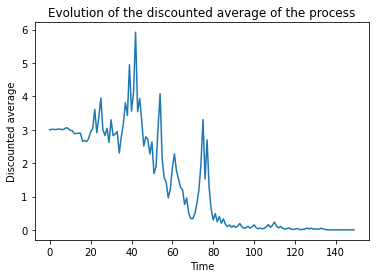
\includegraphics[scale=0.4]{avseed1.png}
\end{minipage}%
\begin{minipage}[b]{.5\textwidth}
  \centering
 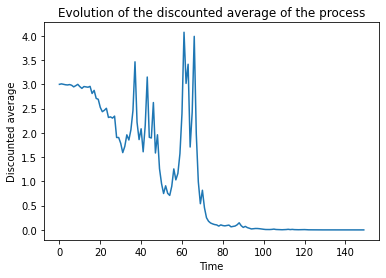
\includegraphics[scale=0.4]{avseed2.png}
\end{minipage}
\end{figure}
\end{frame}

\begin{frame}{Maybe a pure Monte-Carlo approach is not the best solution..}
\begin{itemize}
\item We have seen that, if the volatility is high, the Monte-Carlo approach can be very inaccurate for many time steps.
\item Moreover, it is time consuming (this is a problem common to all brute-force Monte-Carlo approaches) 
\item  \red{Idea:} let us exploit some analytic properties of the Binomial model..
\end{itemize}
\end{frame}


\begin{frame}{Some simple observations}
\begin{itemize}
\item At the $n$-th time step, $n+1$ realizations of the process are possible: $S_0u^n, S_0u^{n-1}d, \dots,  S_0ud^{n-1}, S_0d^{n}$.
\item The number of ups and downs is given by a Bernoulli distribution: 
\blue{$$
P(S_{n}=S_0u^{k}d^{n-k})=\binom{n}{k}q^k(1-p)^{n-k}.
$$}
\item Using the expression above, we can compute
\begin{align}
\blue{\bE^Q[f(S_{n})]}&=\sum_{k=0}^n Q(S_{n}=S_0u^{k}d^{n-k}) f(S_0u^{k}d^{n-k}) \notag \\
&\blue{= \sum_{k=0}^n \binom{n}{k}q^k(1-q)^{n-k}f(S_0u^{k}d^{n-k})}.\notag
\end{align}
\end{itemize}
\end{frame}


\begin{frame}{Implementation in Python}
\begin{itemize}
\item The idea is then to generate all the possible realizations of the process up to a given time, and to weight them by their probability.
\item You can find the code relative to the this approach in
\begin{center}
\texttt{binomialmodel.creationandcalibration.binomialModelSmart},
\end{center}
whose class also extends the one in
\begin{center}
\texttt{binomialmodel.creationandcalibration.binomialModel}.
\end{center}
\item Doing some tests in
\begin{center}
\texttt{binomialmodel.creationandcalibration.binomialModelSmartTest}.
\end{center}
you can observe that, in this way, the average of the discounted process is stable. 
\item Moreover, this approach is of course much faster.
\end{itemize}
\end{frame}

\begin{frame}{Computation of $Q(S_{n}>S_0(1+\rho)^{n})$, $n=1,\dots,T$}
\begin{itemize}
\item Note that for any $k =0, \dots,n$ it holds
\begin{align}
\blue{S_{n}=S_0u^kd^{n-k}>S_0(1+\rho)^{n}}& \iff u^kd^{n-k} > (1+\rho)^n \notag \\
& \iff \left(\frac{u}{d}\right)^k > \left(\frac{1+\rho}{d}\right)^n \notag \\
& \blue{\iff k > n \log_{ \frac{u}{d}} \left(\frac{1+\rho}{d}\right)}. \notag 
\end{align}
\item Then we have
\begin{align}
\red{Q\left(S_{n}>S_0(1+\rho)^{n}\right)}&=\sum_{k=\bar{k}}^n Q(S_{n}=S_0u^{k}d^{n-k}) \notag \\
&\red{=\sum_{k=\bar{k}}^n  \binom{n}{k}q^k(1-q)^{n-k}f(S_0u^{k}d^{n-k})},\notag
\end{align}
where 
\blue{$$
\bar{k}=\min\left\{k \in \mathbb{N}: \ k > n \log_{ \frac{u}{d}} \left(\frac{1+\rho}{d}\right)\right\}\le n.
$$}
\end{itemize}
\end{frame}


\begin{frame}{Evolution of the probability plotted with Python}
We show here the evolution of the probability computed above, over $150$ time steps. 

On the left, we have parameters $S_0=3$, $u=1.1$, $d=0.9$, $\rho=0.1$, $q=\frac{1+\rho-d}{u-d}=0.75$. On the right, $S_0=3$, $u=2$, $d=0.5$, $\rho=0.05$, $q=\frac{1+\rho-d}{u-d}=0.4$.
 \begin{figure}
\centering
\begin{minipage}[b]{.5\textwidth}
  \centering
 \includegraphics[scale=0.4]{probu2.png}
\end{minipage}%
\begin{minipage}[b]{.5\textwidth}
  \centering
 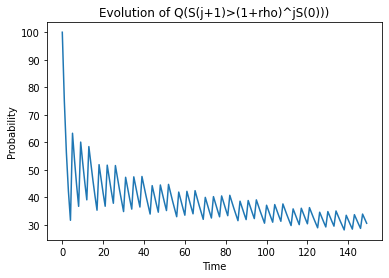
\includegraphics[scale=0.4]{probu11.png}
\end{minipage}
\end{figure}
\end{frame}

\begin{frame}{European option valuation in Python}
\begin{itemize}
\item As seen before, an application of the simulation of the Binomial model in this way is the valuation of European options, under the pricing measure $Q$.
\item In  
\begin{center}
\texttt{binomialmodel.optionValuation.europeanOption},
\end{center}
you can see some methods relative to this.
\item In particular, we compute the expectation of the payoff of European options as
\begin{align}
\blue{\bE^Q[f(S_{n})]}&=\sum_{k=0}^n Q(S_{n}=S_0u^{k}d^{n-k}) f(S_0u^{k}d^{n-k}) \notag \\
&\blue{= \sum_{k=0}^n \binom{n}{k}q^k(1-q)^{n-k}f(S_0u^{k}d^{n-k})}.\notag
\end{align}
\item We also compute the value of a general option for every time $t=0,\dots,T-1$, and the corresponding self-financing, replicating strategy 
$(\alpha_t,\beta_T)$, $t=0,\dots,T-1$, described before.
\item As an exercise, you can check if the final value of the portfolio given by that strategy equals the payoff, for an option of your choice.
\end{itemize}
\end{frame}


\subsection{Calibration of the Binomial model}

\frame{  \tableofcontents[
    sectionstyle=show/shaded,
    subsectionstyle=show/shaded/shaded,
    subsubsectionstyle=show/shaded/shaded/shaded
    ]}


\begin{frame}{Calibration of the parameters $u$ and $d$}
\begin{itemize}
\item Recall that we have
$$
S_t=S_0\cdot Y_1 \cdot \dots \cdot Y_t, \quad t=1,\dots,T,
$$
where 
$$
Y_t = \begin{cases}
u > 1 + \rho \text{ with (risk-neutral) probability $q=\frac{1+\rho-d}{u-d}$} \\
d < 1  \text{ with probability $1-q$}
\end{cases},\quad t=1,\dots,T.
$$
\item Our goal is to \red{calibrate} the up and downs parameters \red{$u$ and $d$}, supposing \blue{we know} the risk neutral probability \blue{$q=\frac{1+\rho-d}{u-d}$} and the interest rate \blue{$\rho>0$}, and that we can observe
\blue{$$
\text{Var}[\log(S_T/S_0)]:=\bE^Q[\log(S_T/S_0)^2]-\bE^Q[\log(S_T/S_0)]^2
$$}
for a given maturity $T$.
\item Observe first that since
$$
\log(S_T/S_0)=\sum_{t=1}^T\log(Y_t), 
$$
and since $(Y_t)_{t=1,\dots,T}$ are equi-distributed, we get
\blue{$$
\text{Var}[\log(S_T/S_0)]=T^2 \text{Var}[\log(Y_T)].
$$}
\end{itemize}
\end{frame}


\begin{frame}{One result about variance}
\begin{block}{Proposition}
Let 
$$
Y_t = \begin{cases}
u > 1 + \rho \text{ with (risk-neutral) probability $q=\frac{1+\rho-d}{u-d}$} \\
d < 1  \text{ with probability $1-q$},
\end{cases},\quad t=1,\dots,T.
$$
Then for any $t=1,\dots,T$ we have 
$$
\text{Var}[\log{Y_t}]=q(1-q)\log(u/d)^2.
$$
\end{block}
\begin{block}{Proof}
\begin{align}
\text{Var}[\log{Y_t}]&=\mathbb{E}^Q[\log(Y_t)^2]-\mathbb{E}^Q[\log(Y_t)]^2 \notag \\
&=\mathbb{E}^Q[\log(Y_t)^2] - (q\log(u)+(1-q)\log(d))^2 \notag \\
&=q\log(u)^2+(1-q)\log(d)^2 \notag \\
& \quad - q^2\log(u)^2 - (1-q)^2\log(d)^2 -  2q(1-q)\log(u)\log(d)\notag \\
&=q(1-q)\log(u)^2+q(1-q)\log(d)^2 -2q(1-q)\log(u)\log(d) \notag \\
&=q(1-q)\left(\log(u)-\log(d)\right)^2 \notag \\
&=q(1-q)\log(u/d)^2.
\end{align}
\end{block}
\end{frame}


\begin{frame}{Calibration with Python}
\begin{itemize}
\item Thanks to 
$$
q=\frac{1+\rho-d}{u-d}
$$
and to
$$
\text{Var}[\log{Y_t}]=q(1-q)\log(u/d)^2,
$$
along with
$$
\sigma_{obs}^2:=\text{Var}[\log(S_T/S_0)]=T^2 \text{Var}[\log(Y_T)],
$$
we can \red{get $u$ and $d$ from $q$, $\rho$ and $\sigma_{obs}^2$} by solving the nonlinear nonsystem
\blue{\begin{equation}\label{eq:system}
\begin{cases}
\frac{1+\rho-d}{u-d}=q \\
\log(u/d)^2 = \frac{\sigma_{obs}^2}{q(1-q)}
\end{cases}
\end{equation}}
\item We can find an approximated solution of \eqref{eq:system} by the \blue{\texttt{fsolve}} function of Python.
\item Look at 
\begin{center}
\texttt{binomialmodel.creationandcalibration.binomialModelCalibration}
\end{center}
to see an implementation of the calibration of $u$ and $d$ as showed above.
\end{itemize}
\end{frame}

\subsection{American options valuation}

\frame{  \tableofcontents[
    sectionstyle=show/shaded,
    subsectionstyle=show/shaded/shaded,
    subsubsectionstyle=show/shaded/shaded/shaded
    ]}

\begin{frame}{American options}
\begin{itemize}
\item The holder of an American option with payoff $f$ and maturity $T$ on an underlying $X$ has the right, at any time we $t\in [0,T]$, to hold the contract or to  exercise the payoff $f(X_t)$.
\item The \blue{valuation of American options is more complicated} than the one of European options, since it involves an optimal exercise problem.
\item In order to valuate such an option at time $t$, indeed, the conditional expectation of the future value of the option at time $t$ has to be computed, and then compared against the present value of the payoff.
\item However, the Monte-Carlo computation of a conditional expectation is very time consuming.
\item One of the \red{strengths of the Binomial model} with respect to other settings is that it \red{permits a favourable pricing of American options}.
\item Also when dealing with continuous time processes, with suitable dynamics, one may approximate them with a Binomial model in order to get the price. 
\end{itemize}
\end{frame}


\begin{frame}{American options valuation under the Binomial model}
\begin{itemize}
\item At any time $t=1,\dots,T$, call $S_t(k)$ and $V_t(k)$ the value of the underlying and of the option, respectively, in the scenario with $k$ ups and $t-k$ downs up to time $t$.
\item Idea: \red{proceed backward}.
\item First we compute the \blue{payoff $f(S_T(k))=f(S_0u^kd^{T-k})$}, for any $k=0,\dots,T$.
\item We have of course \blue{$V_T(k)=f(S_T(k))$}, for any $k=0,\dots,T$.
\item At time $T-1$, for any $k=0,\dots,T-1$ we compute
\begin{align}
\blue{V_{T-1}(k)}&=\max \left( f(S_{T-1}(k)),\frac{1}{1+\rho}\left(q V_{T}(k+1)+(1-q)V_{T}(k)\right)\right)\notag \\
&=\blue{\max \left( f(S_0u^k d^{T-1-k}),\frac{1}{1+\rho}\left(q V_{T}(k+1)+(1-q)V_{T}(k)\right)\right)}.\notag
\end{align}
\item For any $t=1,\dots, T-2$ we compute with the same argument
\blue{$$
V_{t}(k)=\max \left( f(S_0u^kd^{t-k}),\frac{1}{1+\rho}\left(q V_{t}(k+1)+(1-q)V_{t}(k)\right)\right).\notag
$$}
\item We finally get the value of the option at initial time as
\blue{$$
V_0= \max \left( f(S_0),\frac{1}{1+\rho}\left(q V_{1}(1)+(1-q)V_{1}(0)\right)\right).
$$}
\end{itemize}
\end{frame}


\begin{frame}{Implementation in Python}
You can find the code relative to the the valuation of American options in
\begin{center}
\texttt{binomialmodel.optionValuation.AmericanOption},
\end{center}
with some tests in 
\begin{center}
\texttt{binomialmodel.optionValuation.AmericanOptionTest},
\end{center}
\end{frame}

\begin{frame}{Example}
We consider a put option with payoff $f(x)=(20-x)^+$, and choose parameters $T=3$, $S_0=20$, $u=1.1$, $d=0.9$, $\rho=0.05$. 

The triangular matrices below show us an analysis of an American option for the such parameters (row 3 shows the values for $t=3$ and so on). 

The upper left and upper right matrices show the amount one would get if exercising the option or holding the contract, respectively; the lower left one the values of the option; the lower right one has $1$ in the exercise region and $0$ in the hold region
 \begin{figure}
\centering
\begin{minipage}[b]{.5\textwidth}
  \centering
 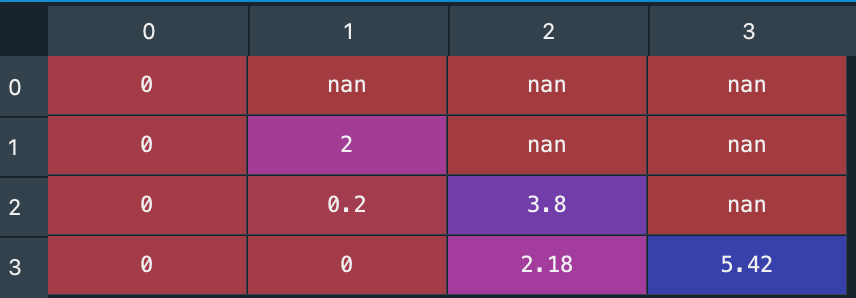
\includegraphics[scale=0.4]{valueExercise.png}
\end{minipage}%
\begin{minipage}[b]{.5\textwidth}
  \centering
 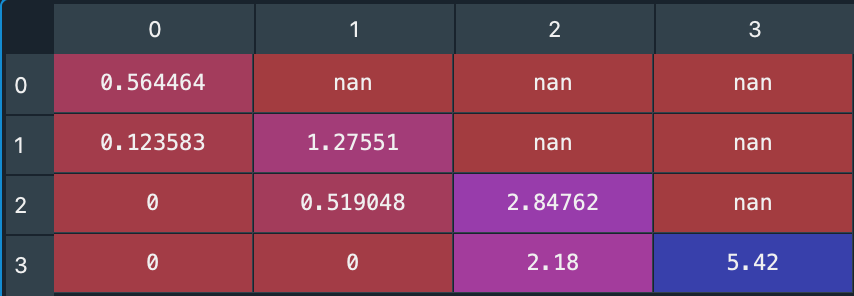
\includegraphics[scale=0.4]{valueWait.png}
\end{minipage}
\end{figure}
 \begin{figure}
\centering
\begin{minipage}[b]{.5\textwidth}
  \centering
 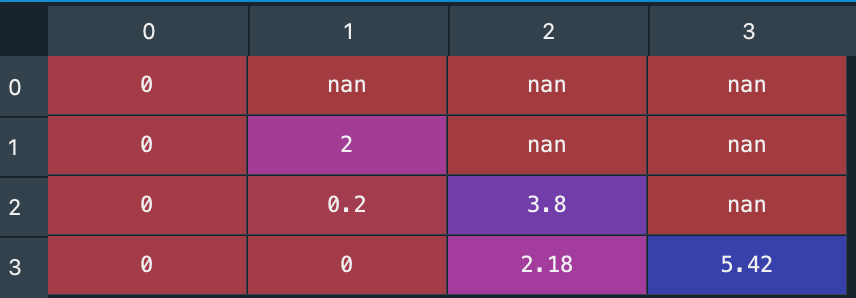
\includegraphics[scale=0.4]{valueExercise.png}
\end{minipage}%
\begin{minipage}[b]{.5\textwidth}
  \centering
 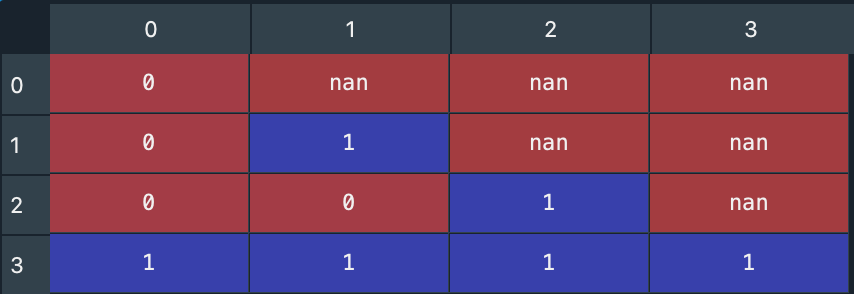
\includegraphics[scale=0.4]{exercise}
\end{minipage}
\end{figure}
\end{frame}

\begin{frame}{Approximating a Black-Scholes model with a Binomial model}
\begin{itemize}
\item Consider a continuous, adapted stochastic process $X=(X_t)_{t \ge 0}$ with dynamics 
\blue{$$
dX_t=r X_t dt + \sigma X_t dW_t, \quad t \ge 0,
$$}
where $r,\sigma>0$ and $W=(W_t)_{t \ge 0}$ is a Brownian motion. 
\item Suppose you want to price an American option with underlying $X$ and maturity $T > 0$.
\item It can be seen that the dynamics of \red{$X=(X_t)_{0 \le t  \le T}$} can be \red{approximated by $N$ time steps of a Binomial model with parameters
\begin{equation}\label{eq:parameters}
u = e^{\sigma \sqrt{T/N}}, \qquad d=1/d, \qquad \rho = e^{r \sqrt{T/N}},
\end{equation}
for $N$ large enough}, see for example .
\item The idea is to \red{approximate the price of the American option} of maturity $T$ with the price of an American option with maturity $N$ written a Binomial model with parameters as in \eqref{eq:parameters}, for $N$ large enough.
\item Indeed, the price of the American option written on the Binomial model can be found as illustrated before.
\end{itemize}
\end{frame}

\begin{frame}{Example: not such a nice behaviour}
We consider an American put option with payoff $f(x)=(1-x)^+$ and maturity $T=3$, written on a Black-Scholes model with parameters $r=0.02$, $\sigma=0.7$.

The plot below shows the approximated price via the derivation under the Binomial model, for an increasing number of times steps up to $N=150$.  
 \begin{figure}
\centering
 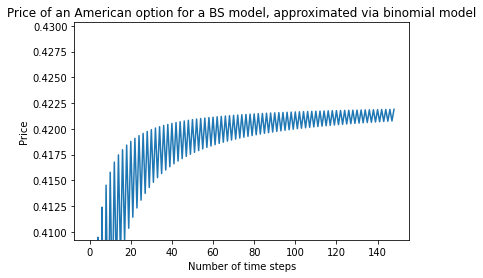
\includegraphics[scale=0.65]{american.png}
\end{figure}
\end{frame}


\begin{frame}{Control variates for American call and put options}
\begin{itemize}
\item \red{First idea}: \blue{we know the analytic price of an European put} (or call) option under the Black-Scholes model. For example, call \blue{$P^E$} the Black-Scholes formula price of an European put option.
\item Also call:
\begin{itemize}
\item $P^E_N$ the price of an European put approximated by the Binomial model with $N$ time steps;
\item $P^A$ the analytic price of an American put;
\item $P^A_N$ the price of an American put approximated by the Binomial model with $N$ time steps.
\end{itemize}
\item \red{Second idea}: we know the euristics \blue{$P^A-P^A_N \approx P^E-P^E_N$}.
\item We then approximate
$$
\red{P^A \approx P^A_N + (P^E-P^E_N)}
$$
\item This approximates the price of an American put option via control variates.
\item Same thing for a call option.
\end{itemize}
\end{frame}

\begin{frame}{A nicer behaviour with control variates}
We consider again an American put option with payoff $f(x)=(1-x)^+$ and maturity $T=3$, written on a Black-Scholes model with parameters $r=0.02$, $\sigma=0.7$: same situation as before

The plot below compares the prices introduced in the previous slide, for an increasing number of times steps up to $N=150$.  
 \begin{figure}
\centering
 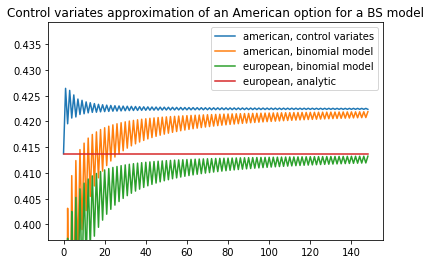
\includegraphics[scale=0.65]{americancv.png}
\end{figure}
\end{frame}

\begin{frame}{Implementation in Python}
\begin{itemize}
\item You can find some experiments relative to the stability of approximations of prices of American options with the Binomial model in
\begin{center}
\texttt{binomialmodel.optionValuation.AmericanOptionPriceConvergence},
\end{center}
\item The code performing the control variates approach can be found in
\begin{center}
\texttt{binomialmodel.optionValuation.controlVariates},
\end{center}
with some tests in 
\begin{center}
\texttt{binomialmodel.optionValuation.controlVariatesTest}.
\end{center}
\end{itemize}
\end{frame}


\end{document}




%``



